\begin{appendices}

\chapter{Analyzing Synthetic Data}
Here we provide additional visualizations which we generated for the purpose of our thesis for synthetic data analysis of \textit{growing networks} in section \ref{growing_networks}.

As we have detailed in algorithm \ref{growing_network_model}, we grow the synthetic networks for $t(=10000)$ iterations in our experiments for \textit{Growing Networks}. We visualize the change in count of minority and majority nodes in the recommendation list of length $k(=5)$ for recommendations to minority and majority nodes with progress in time. The iteration step-size considered for these plots is 1000.

Also for the \textit{reinforcement methods} we only provide the results for the ranking factor $r=1.0$ in the results section for \textit{growing networks}. Here we provide the additional plots for the ranking factor values of $r=\{0.0, 0.5\}$ for the \textit{Ranked-Bandit} and \textit{Top-Rank} recommender methods.

%\section{Experimental Results : PA-Homophily}

\begin{figure}[h!]
	\centering
	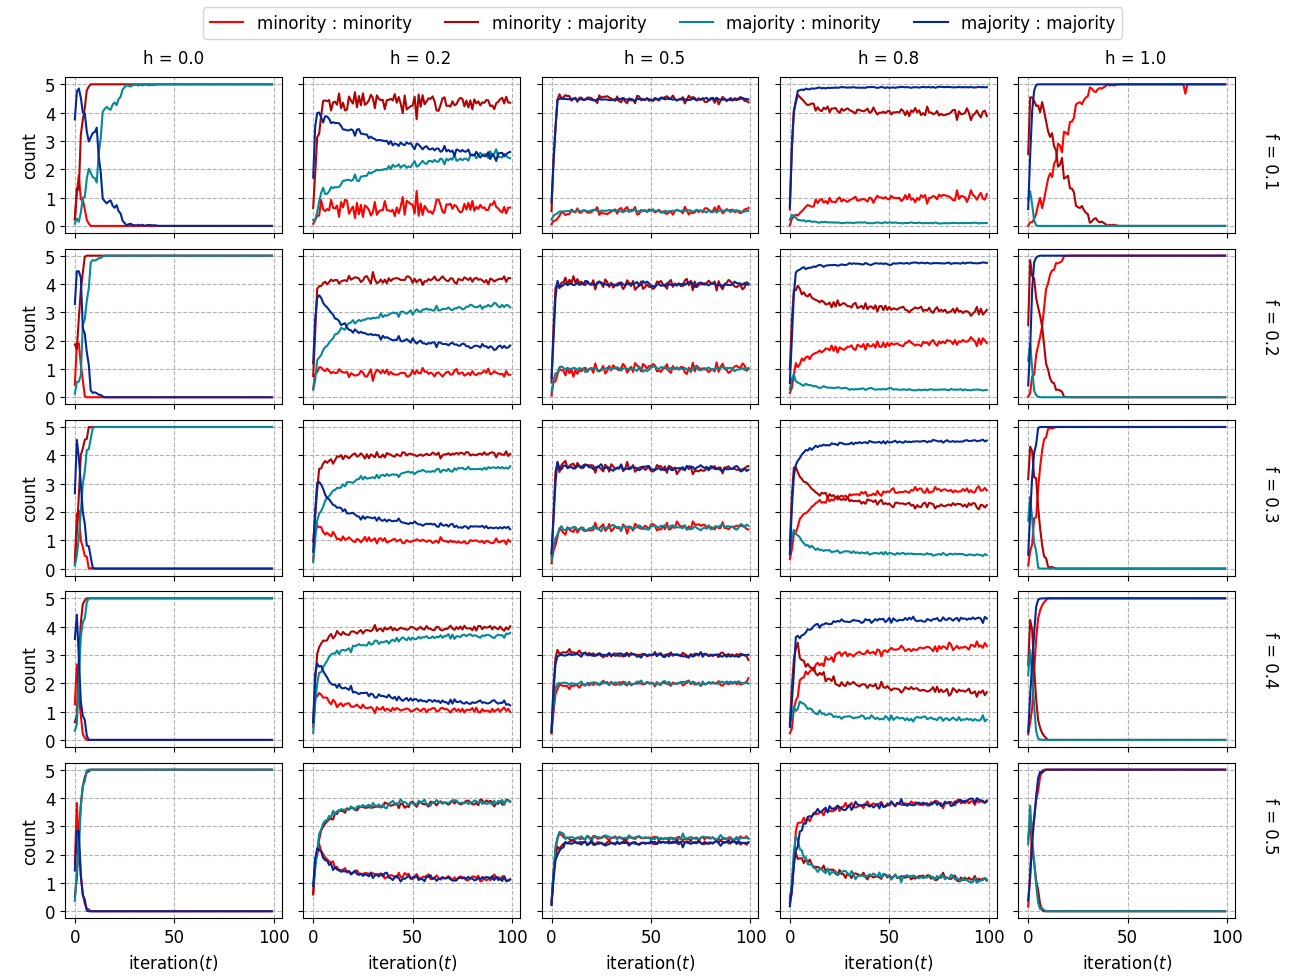
\includegraphics[width=1.0\textwidth]{images/count_pa.png}
	\caption{Count of nodes in the recommendation list over time for minority and majority nodes in a growing network aided with \textbf{PA-Homophily} recommender agent. Homophily values are specified above the respective columns and minority fractions are specified at the right side of the row. Light red plot line denotes count of minority nodes recommended for other minority nodes. Dark red plot line denotes count of majority nodes recommended for other minority nodes. Light blue line denotes count of minority nodes recommended for other majority nodes. Dark blue line denotes count of majority nodes recommended for other majority nodes.}
	\label{count_pa}
\end{figure}

%\section{Experimental Results : Adamic-Adar}

\begin{figure}[h!]
	\centering
	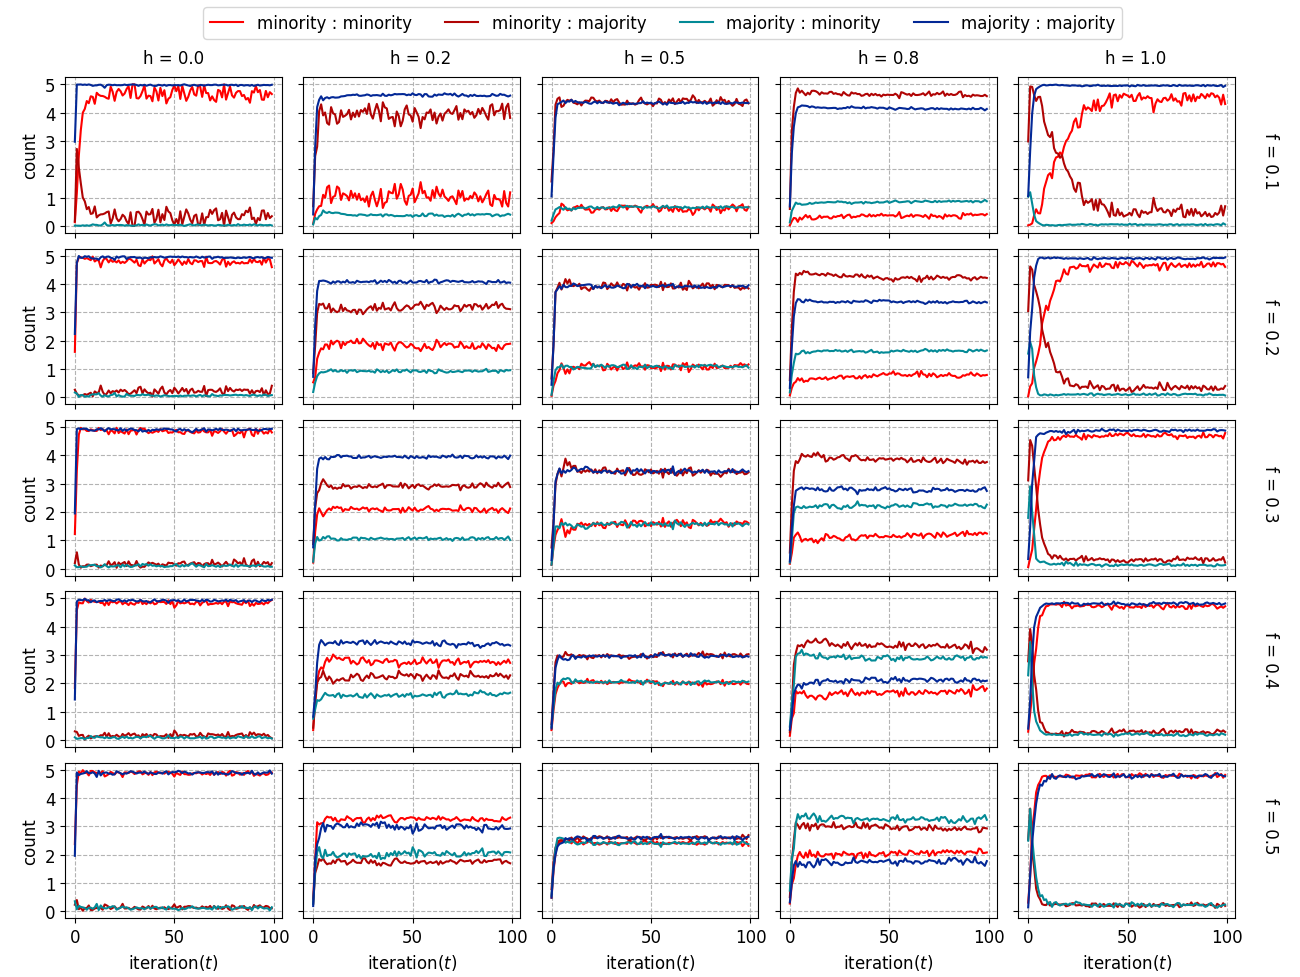
\includegraphics[width=1.0\textwidth]{images/count_aa.png}
	\caption{Count of nodes in the recommendation list over time for minority and majority nodes in a growing network aided with \textbf{Adamic-Adar} recommender agent. Homophily values are specified above the respective columns and minority fractions are specified at the right side of the row. Light red plot line denotes count of minority nodes recommended for other minority nodes. Dark red plot line denotes count of majority nodes recommended for other minority nodes. Light blue line denotes count of minority nodes recommended for other majority nodes. Dark blue line denotes count of majority nodes recommended for other majority nodes.}
	\label{count_aa}
\end{figure}

%\section{Experimental Results : Twitter-Rank}

\begin{figure}[h!]
	\centering
	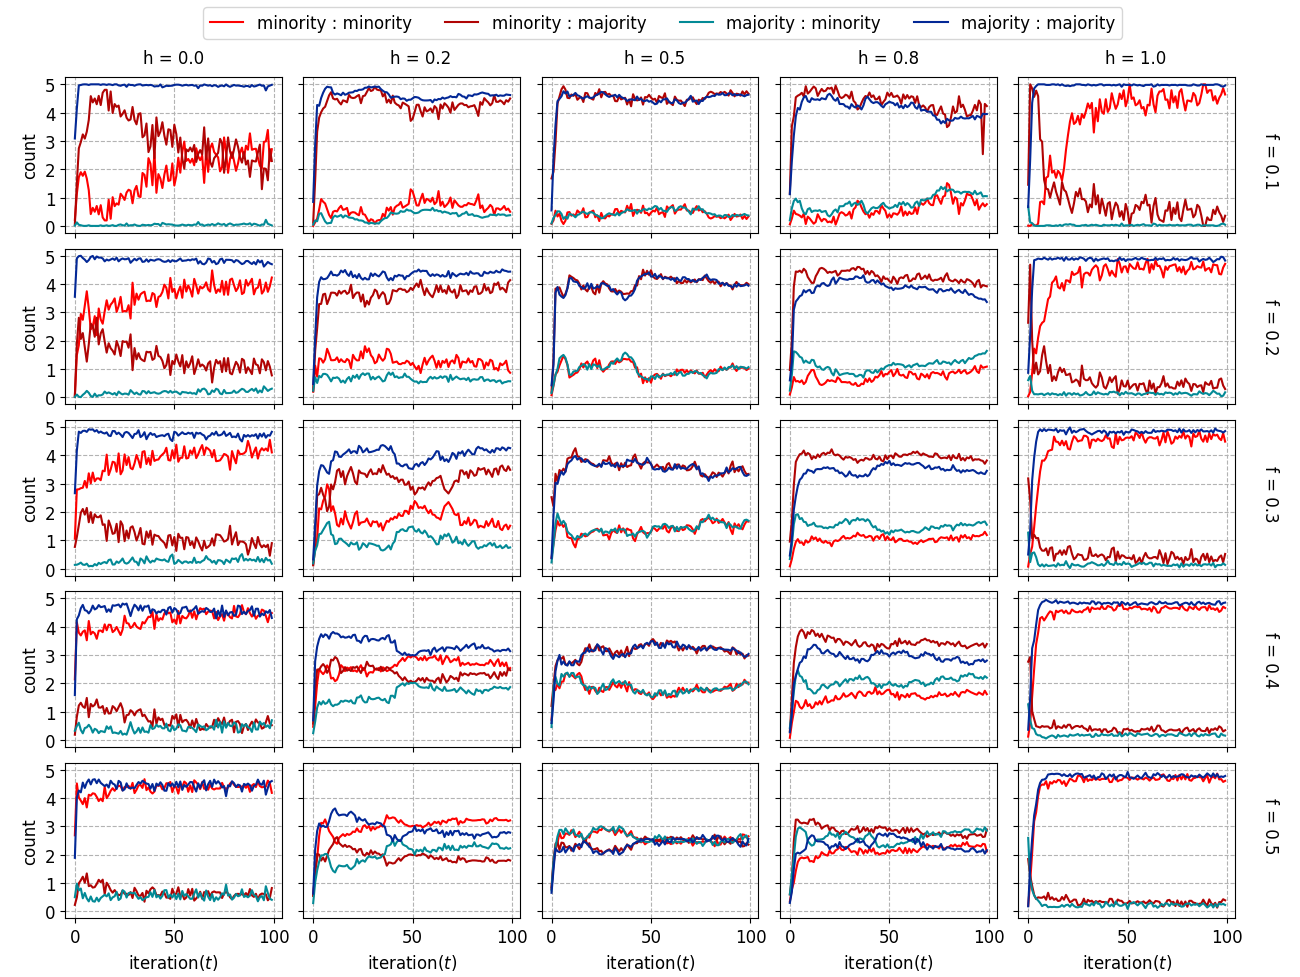
\includegraphics[width=1.0\textwidth]{images/count_tr.png}
	\caption{Count of nodes in the recommendation list over time for minority and majority nodes in a growing network aided with \textbf{Twitter-Rank} recommender agent. Homophily values are specified above the respective columns and minority fractions are specified at the right side of the row. Light red plot line denotes count of minority nodes recommended for other minority nodes. Dark red plot line denotes count of majority nodes recommended for other minority nodes. Light blue line denotes count of minority nodes recommended for other majority nodes. Dark blue line denotes count of majority nodes recommended for other majority nodes.}
	\label{count_tr}
\end{figure}

%\section{Experimental Results : Ranked-Bandit (r=0.0)}

\begin{figure}[h!]
	\centering
	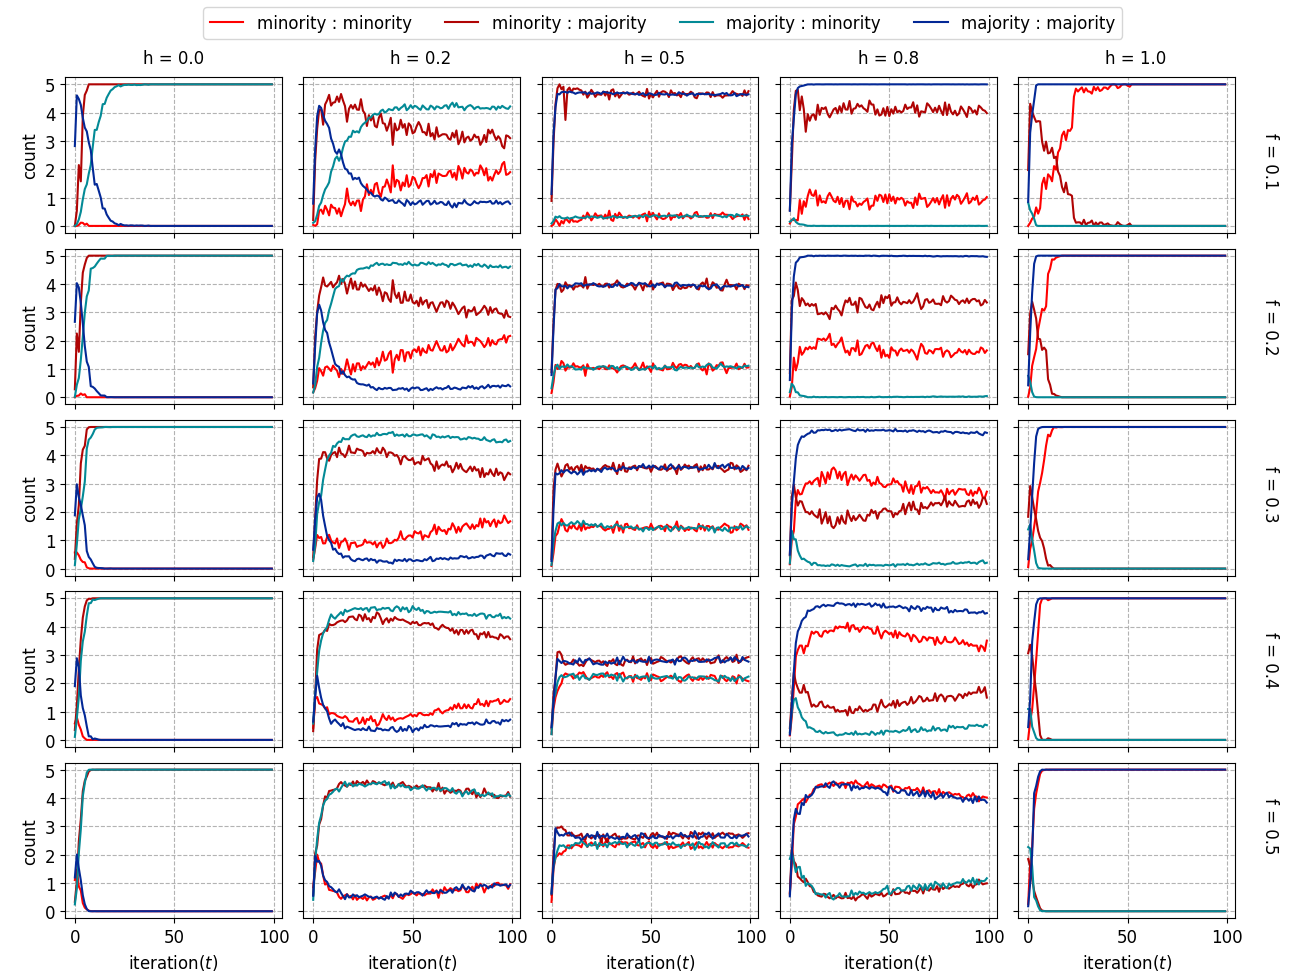
\includegraphics[width=1.0\textwidth]{images/count_rb00.png}
	\caption{Count of nodes in the recommendation list over time for minority and majority nodes in a growing network aided with \textbf{Ranked-Bandit}(r=0.0) recommender agent. Homophily values are specified above the respective columns and minority fractions are specified at the right side of the row. Light red plot line denotes count of minority nodes recommended for other minority nodes. Dark red plot line denotes count of majority nodes recommended for other minority nodes. Light blue line denotes count of minority nodes recommended for other majority nodes. Dark blue line denotes count of majority nodes recommended for other majority nodes.}
	\label{count_rb00}
\end{figure}

\begin{figure}[h!]
	\centering
	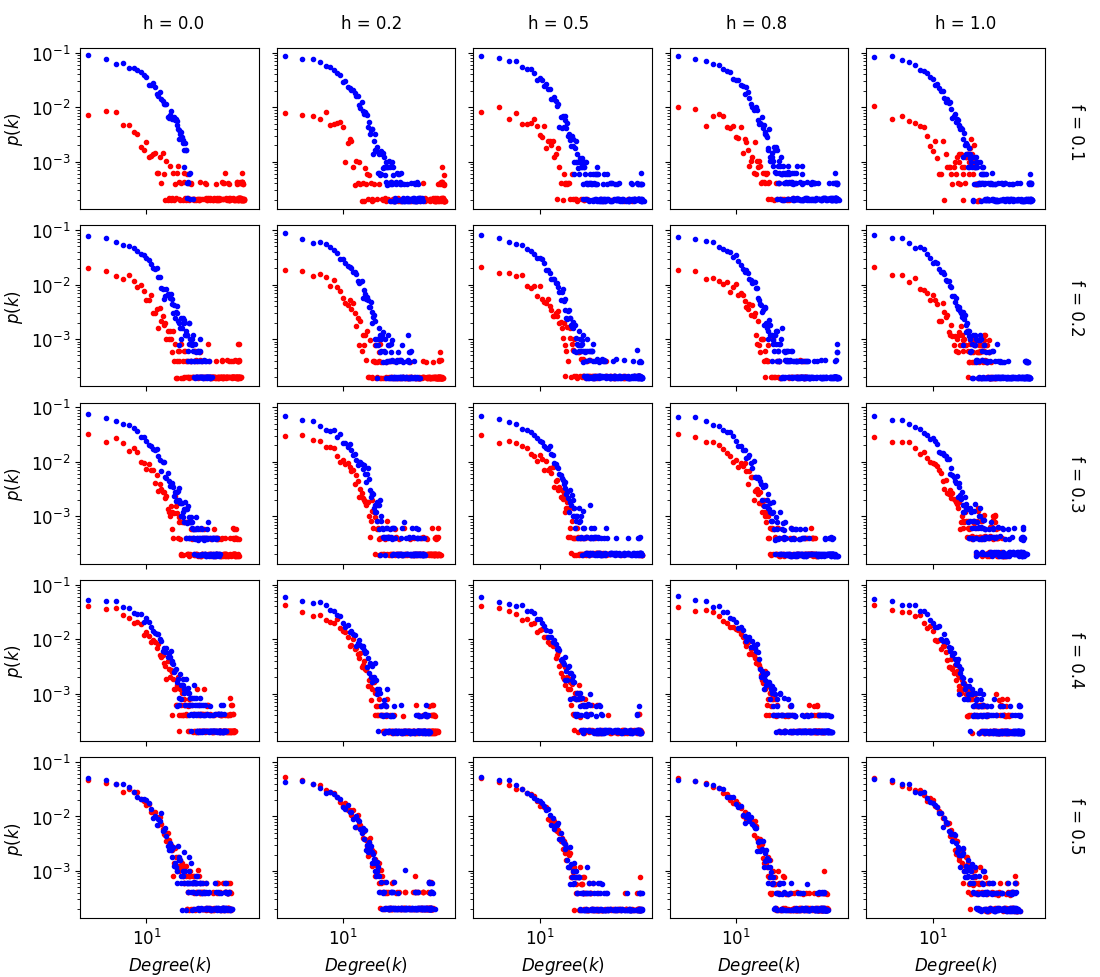
\includegraphics[width=1.0\textwidth]{images/dd_growth_rb00.png}
	\caption{Degree distribution for growing networks with \textbf{Ranked-Bandit ($r = 0.0$)}.The minority fractions are provided at the right-side of each row and the homophily values are specified at the top of each column. Degree distribution for the majority and minority nodes are visualized using blue and red plot points respectively.}
	\label{dd_growth_rb00_fig}
\end{figure}

\begin{figure}[h!]
	\centering
	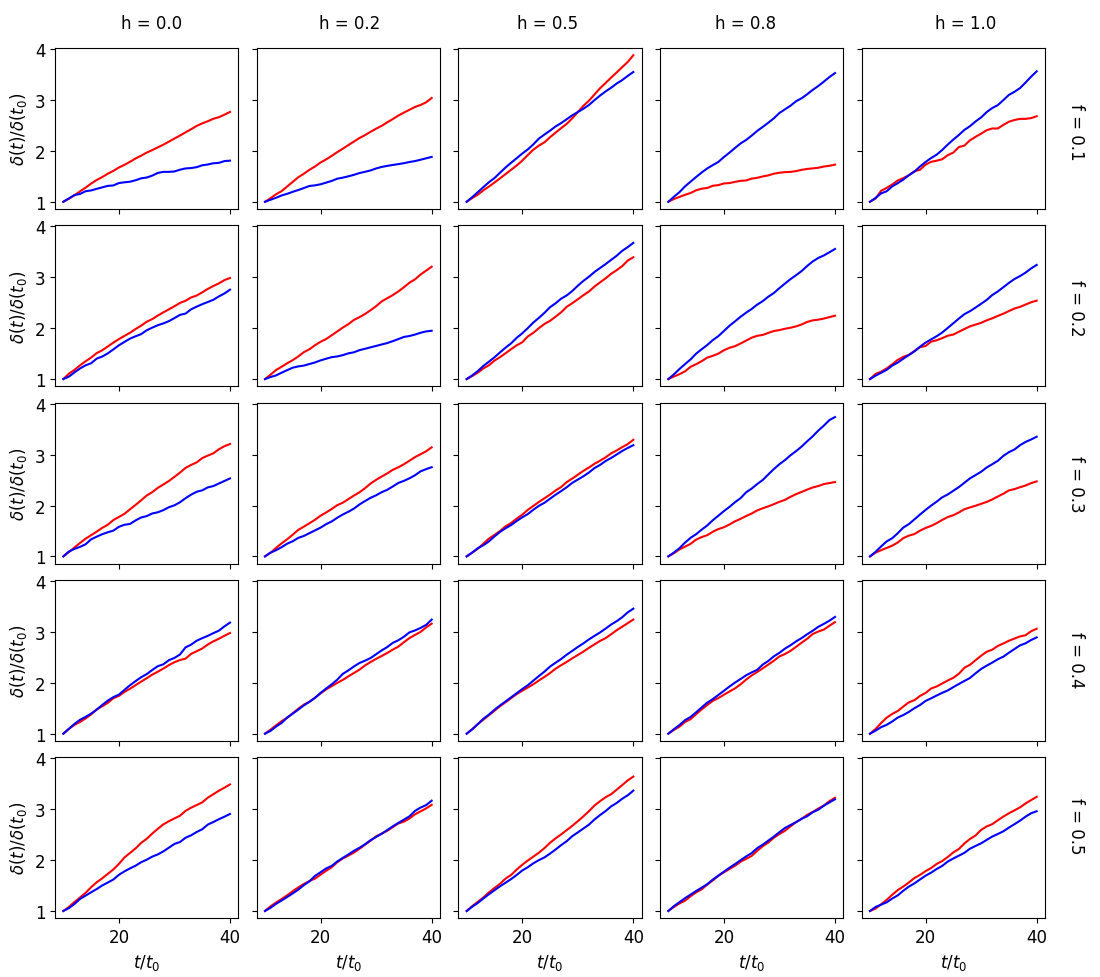
\includegraphics[width=1.0\textwidth]{images/dg_growth_rb00.png}
	\caption{Degree growth for growing networks with \textbf{Ranked-Bandit ($r = 0.0$)}. The minority fractions are provided at the right-side of each row and the homophily values are specified at the top of each column. Degree growth for minority and majority node is visualized using red and blue color plot lines respectively.}
	\label{dg_growth_rb00_fig}
\end{figure}

\begin{SCfigure}[1][h!]
	\centering
	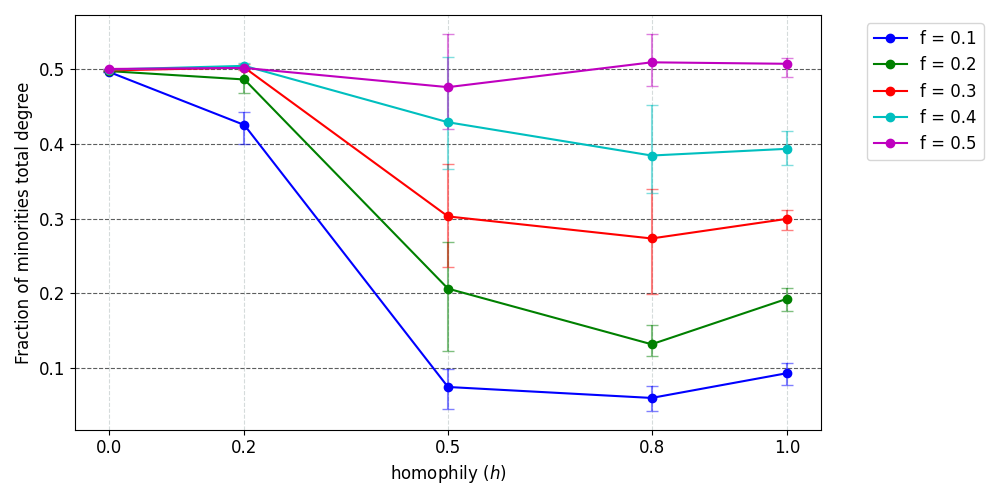
\includegraphics[trim=0 5 0 10, clip, width=0.75\textwidth]{images/mf_growth_rb00.png}
	\caption{The fraction of total degree held by minority nodes for growing networks with \textbf{Ranked-Bandit ($r = 0.0$)}.}
	\label{mf_growth_rb00_fig}
\end{SCfigure}

\begin{figure}[h!]
	\centering
	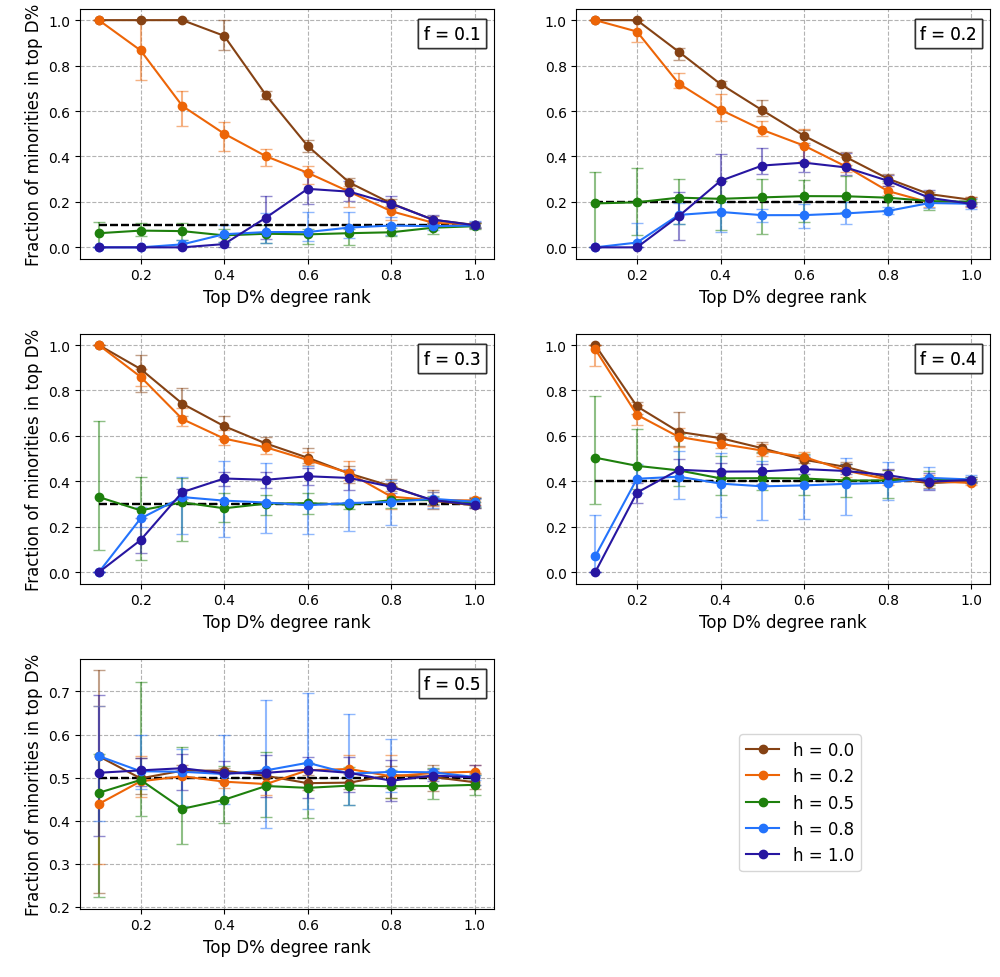
\includegraphics[trim=0 10 0 5, clip, width=1.0\textwidth]{images/top_growth_rb00.png}
	\caption{The fraction of minority nodes found in top D\% nodes ranked according to degree in growing networks with \textbf{Ranked-Bandit ($r = 0.0$)}. A black dotted line at each plot shows the actual fraction of minority nodes in the network.}
	\label{top_growth_rb00_fig}
\end{figure}

%\section{Experimental Results : Ranked-Bandit (r=0.5)}

\begin{figure}[h!]
	\centering
	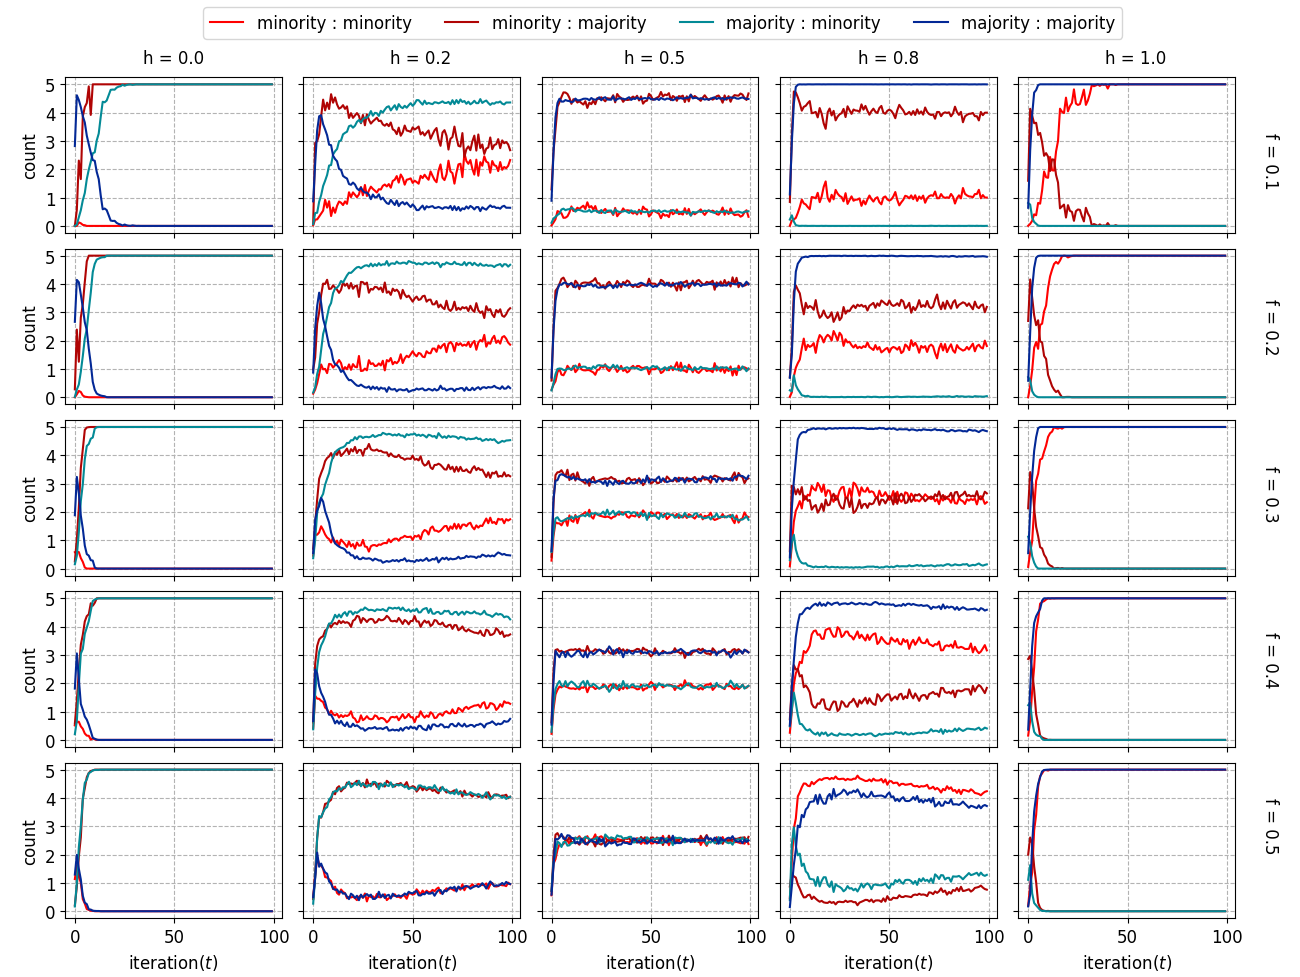
\includegraphics[width=1.0\textwidth]{images/count_rb05.png}
	\caption{Count of nodes in the recommendation list over time for minority and majority nodes in a growing network aided with \textbf{Ranked-Bandit}(r=0.5) recommender agent. Homophily values are specified above the respective columns and minority fractions are specified at the right side of the row. Light red plot line denotes count of minority nodes recommended for other minority nodes. Dark red plot line denotes count of majority nodes recommended for other minority nodes. Light blue line denotes count of minority nodes recommended for other majority nodes. Dark blue line denotes count of majority nodes recommended for other majority nodes.}
	\label{count_rb05}
\end{figure}

\begin{figure}[h!]
	\centering
	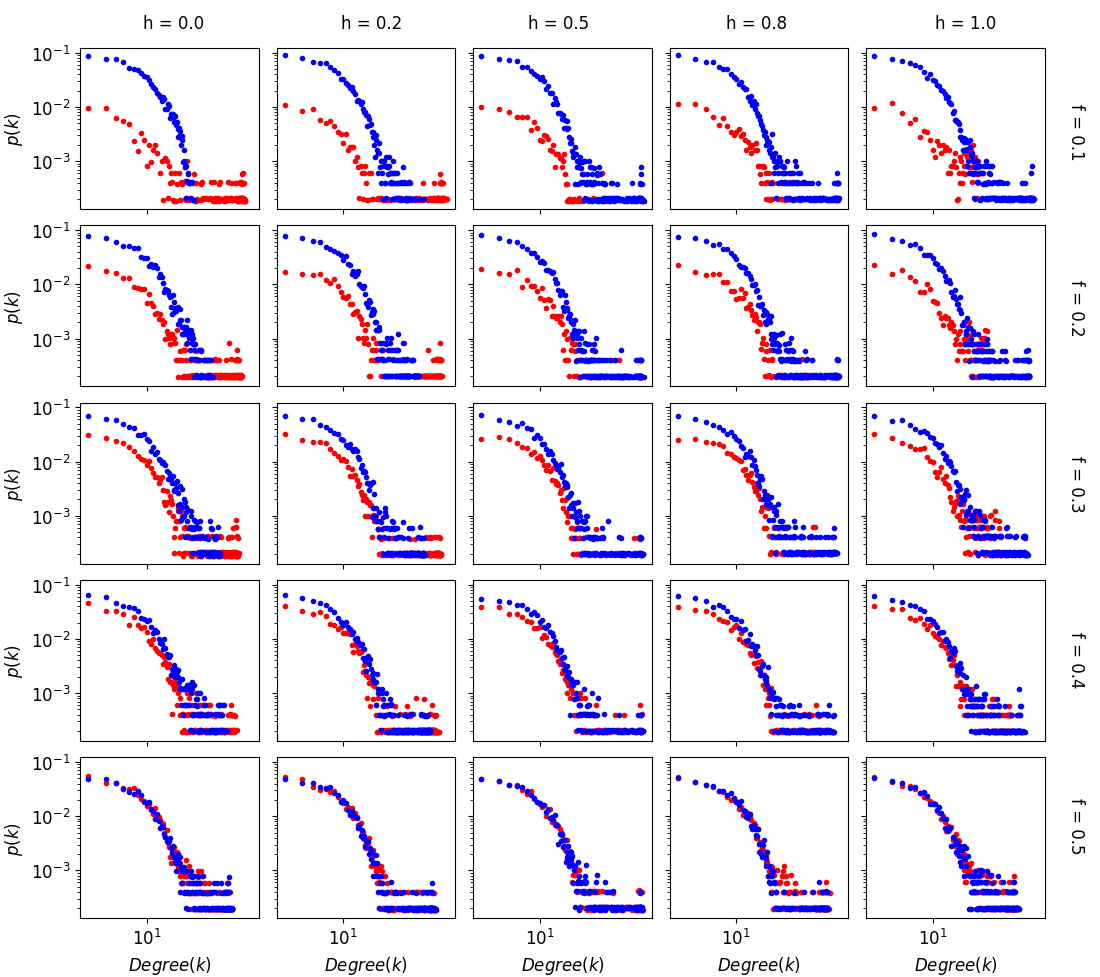
\includegraphics[width=1.0\textwidth]{images/dd_growth_rb05.png}
	\caption{Degree distribution for growing networks with \textbf{Ranked-Bandit ($r = 0.5$)}.The minority fractions are provided at the right-side of each row and the homophily values are specified at the top of each column. Degree distribution for the majority and minority nodes are visualized using blue and red plot points respectively.}
	\label{dd_growth_rb05_fig}
\end{figure}

\begin{figure}[h!]
	\centering
	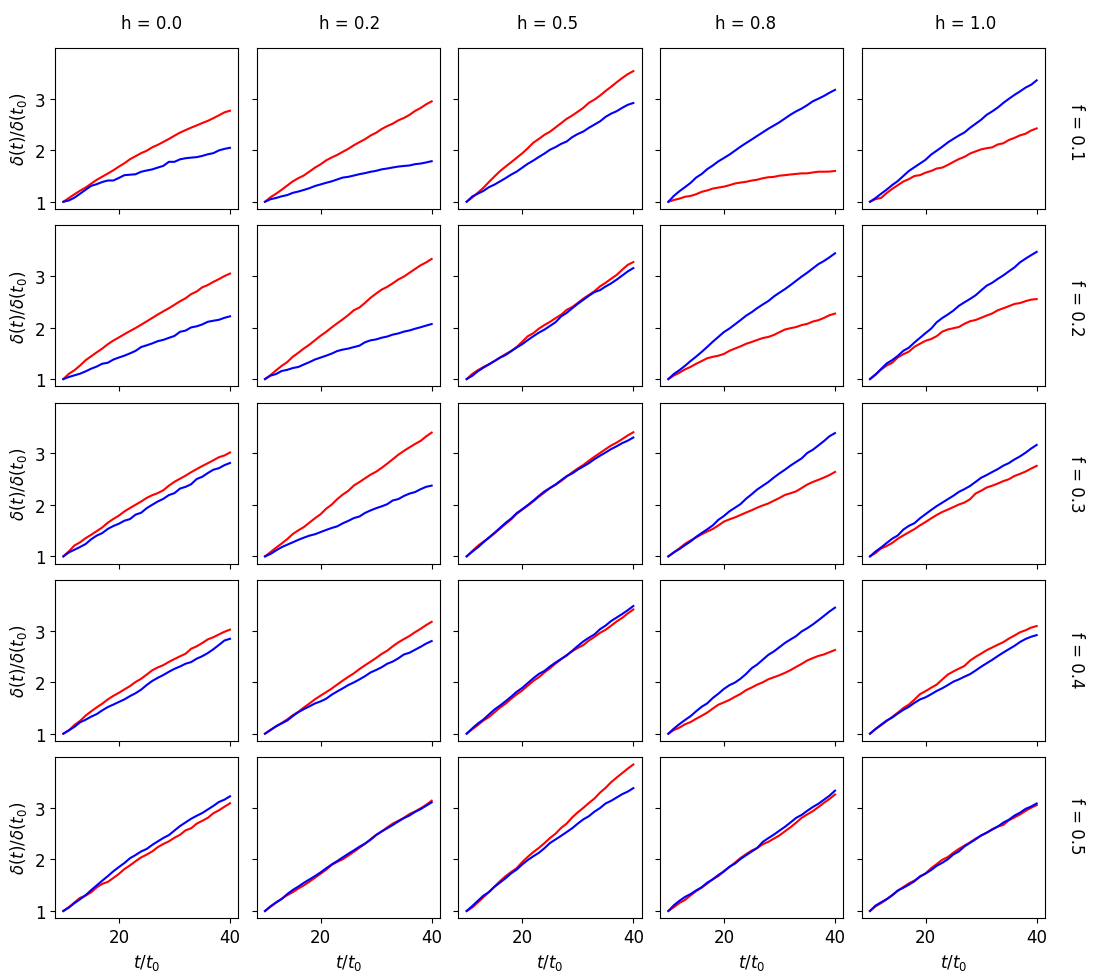
\includegraphics[width=1.0\textwidth]{images/dg_growth_rb05.png}
	\caption{Degree growth for growing networks with \textbf{Ranked-Bandit ($r = 0.5$)}. The minority fractions are provided at the right-side of each row and the homophily values are specified at the top of each column. Degree growth for minority and majority node is visualized using red and blue color plot lines respectively.}
	\label{dg_growth_rb05_fig}
\end{figure}

\begin{SCfigure}[1][h!]
	\centering
	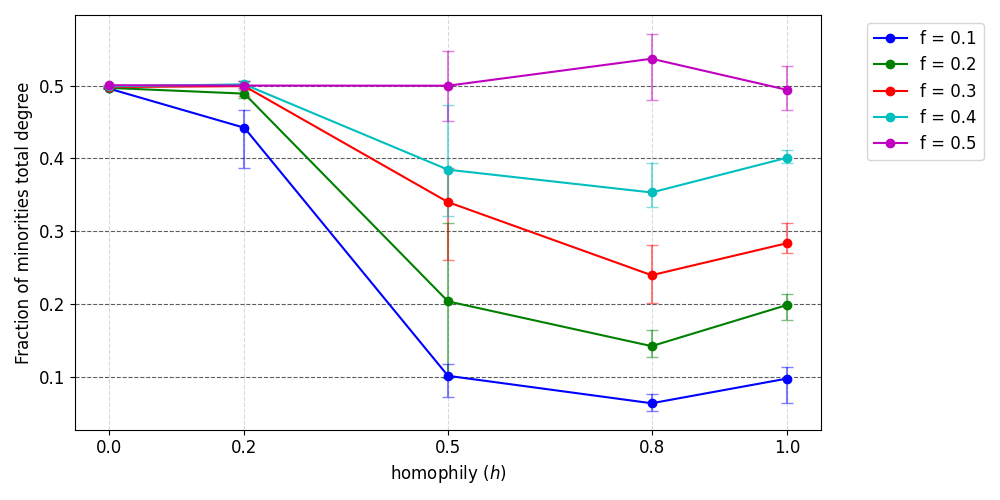
\includegraphics[trim=0 5 0 10, clip, width=0.75\textwidth]{images/mf_growth_rb05.png}
	\caption{The fraction of total degree held by minority nodes for growing networks with \textbf{Ranked-Bandit ($r = 0.5$)}.}
	\label{mf_growth_rb05_fig}
\end{SCfigure}

\begin{figure}[h!]
	\centering
	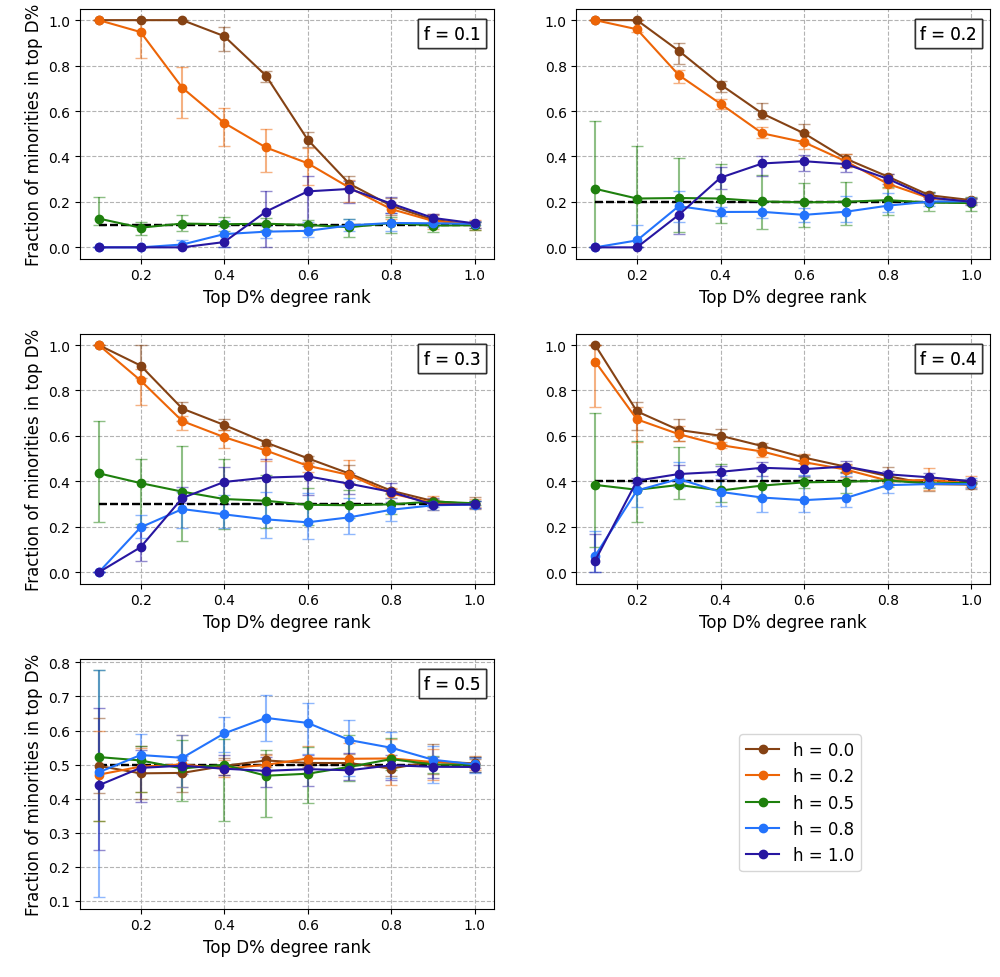
\includegraphics[trim=0 10 0 5, clip, width=1.0\textwidth]{images/top_growth_rb05.png}
	\caption{The fraction of minority nodes found in top D\% nodes ranked according to degree in growing networks with \textbf{Ranked-Bandit ($r = 0.5$)}. A black dotted line at each plot shows the actual fraction of minority nodes in the network.}
	\label{top_growth_rb05_fig}
\end{figure}

%\section{Experimental Results : Ranked-Bandit (r=1.0)}

\begin{figure}[h!]
	\centering
	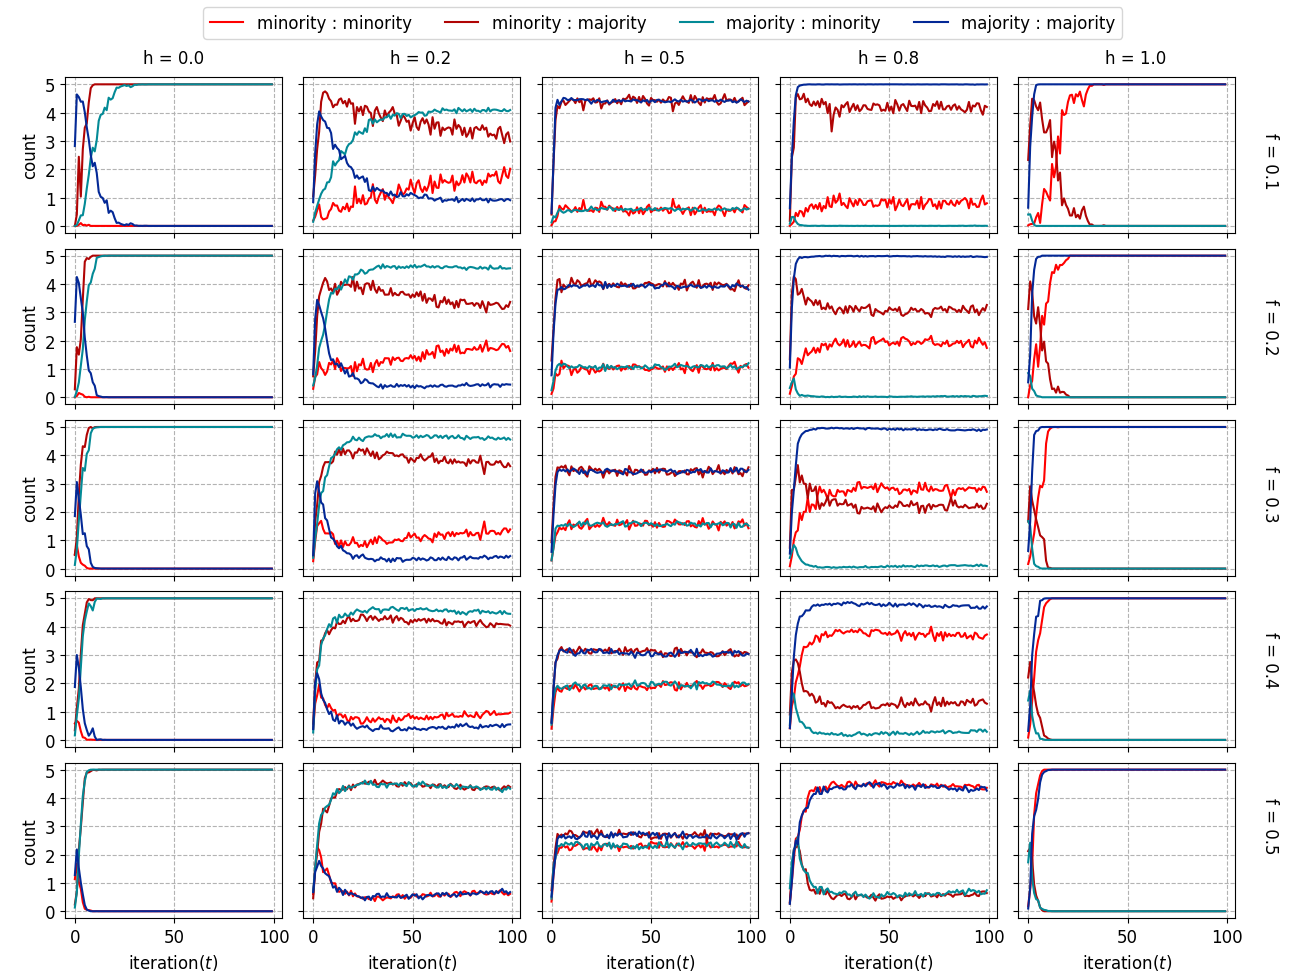
\includegraphics[width=1.0\textwidth]{images/count_rb10.png}
	\caption{Count of nodes in the recommendation list over time for minority and majority nodes in a growing network aided with \textbf{Ranked-Bandit}(r=1.0) recommender agent. Homophily values are specified above the respective columns and minority fractions are specified at the right side of the row. Light red plot line denotes count of minority nodes recommended for other minority nodes. Dark red plot line denotes count of majority nodes recommended for other minority nodes. Light blue line denotes count of minority nodes recommended for other majority nodes. Dark blue line denotes count of majority nodes recommended for other majority nodes.}
	\label{count_rb10}
\end{figure}

%\section{Experimental Results : Top-Rank (r=0.0)}

\begin{figure}[h!]
	\centering
	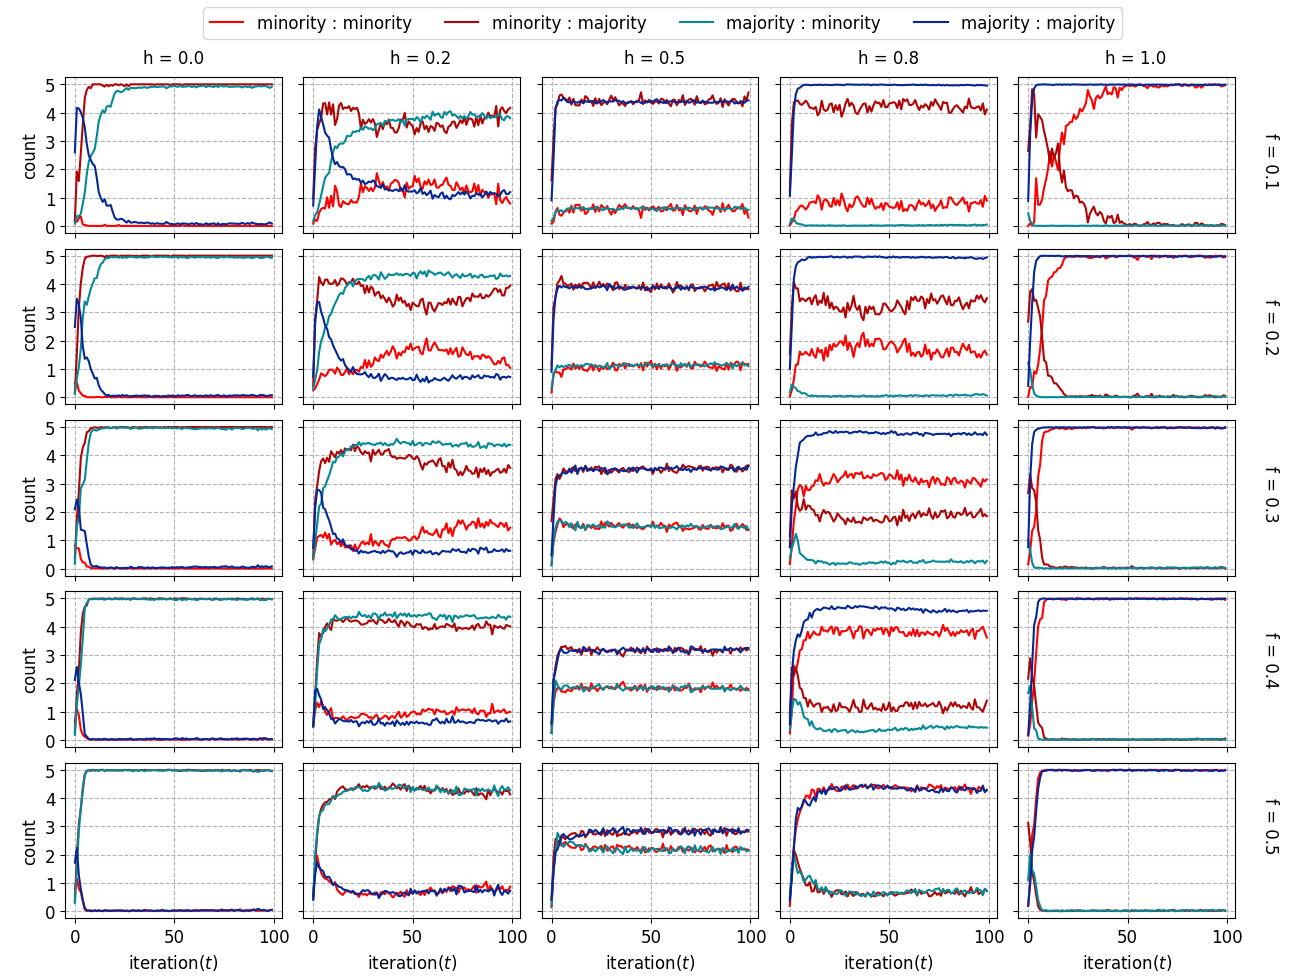
\includegraphics[width=1.0\textwidth]{images/count_top00.png}
	\caption{Count of nodes in the recommendation list over time for minority and majority nodes in a growing network aided with \textbf{Top-Rank}(r=0.0) recommender agent. Homophily values are specified above the respective columns and minority fractions are specified at the right side of the row. Light red plot line denotes count of minority nodes recommended for other minority nodes. Dark red plot line denotes count of majority nodes recommended for other minority nodes. Light blue line denotes count of minority nodes recommended for other majority nodes. Dark blue line denotes count of majority nodes recommended for other majority nodes.}
	\label{count_top00}
\end{figure}

\begin{figure}[h!]
	\centering
	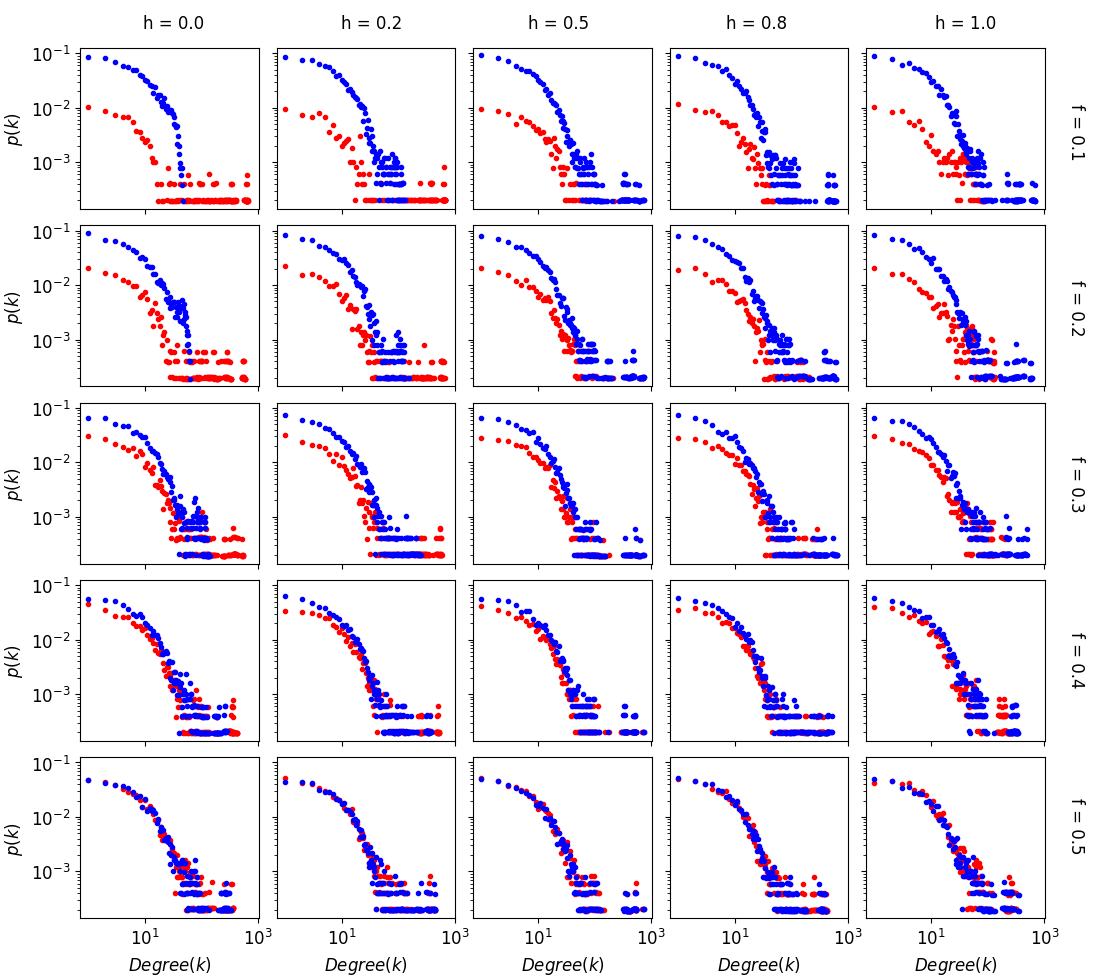
\includegraphics[width=1.0\textwidth]{images/dd_growth_top00.png}
	\caption{Degree distribution for growing networks with \textbf{Top-Rank ($r = 0.0$)}. The minority fractions are provided at the right-side of each row and the homophily values are specified at the top of each column. Degree distribution for the majority and minority nodes are visualized using blue and red plot points respectively.}
	\label{dd_growth_top00_fig}
\end{figure}

\begin{figure}[h!]
	\centering
	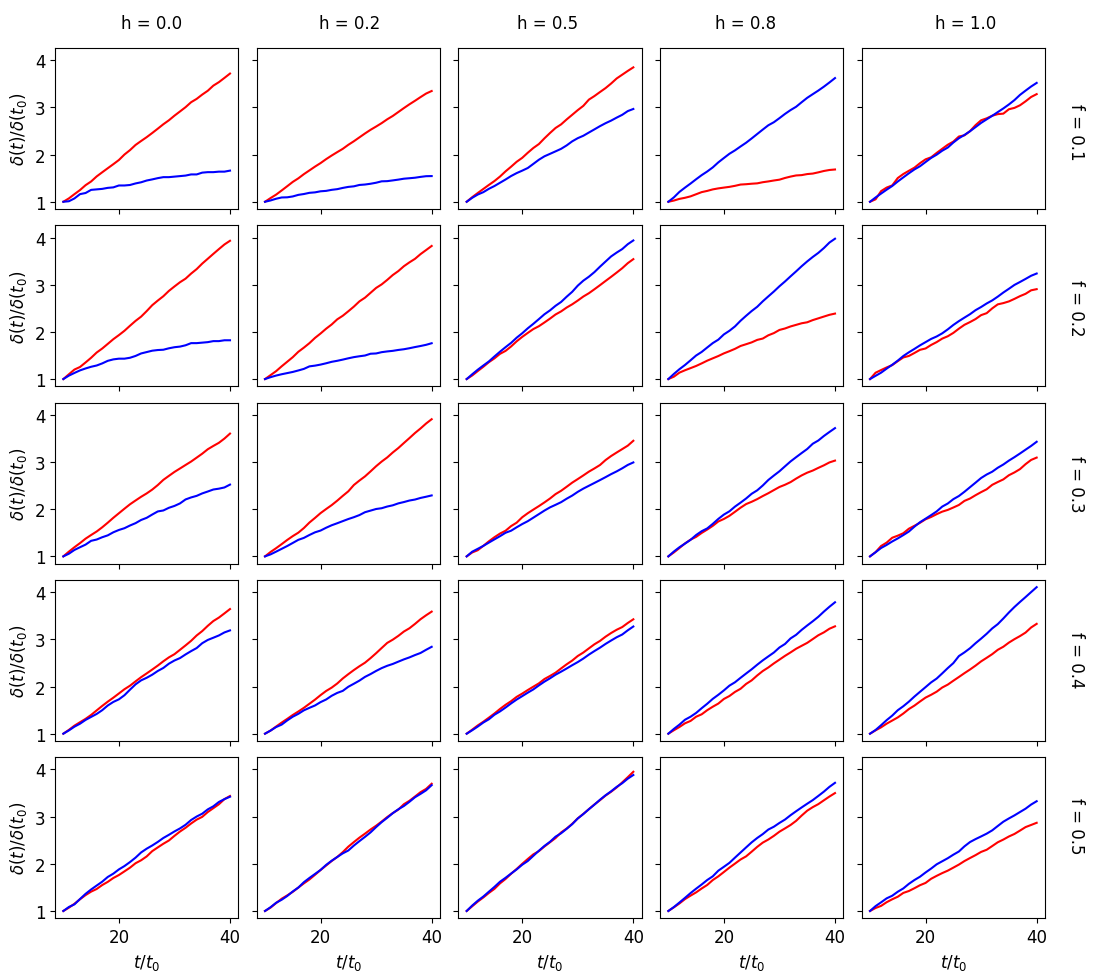
\includegraphics[width=1.0\textwidth]{images/dg_growth_top00.png}
	\caption{Degree growth for growing networks with \textbf{Top-Rank ($r = 0.0$)}. The minority fractions are provided at the right-side of each row and the homophily values are specified at the top of each column. Degree growth for minority and majority node is visualized using red and blue color plot lines respectively.}
	\label{dg_growth_top00_fig}
\end{figure}

\begin{SCfigure}[1][h!]
	\centering
	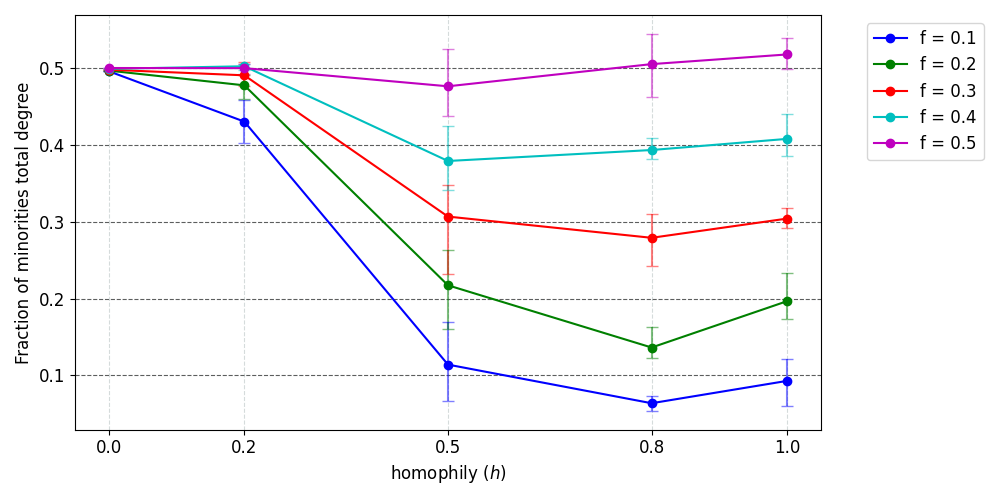
\includegraphics[trim=0 5 0 10, clip, width=0.75\textwidth]{images/mf_growth_top00.png}
	\caption{The fraction of total degree held by minority nodes for growing networks with \textbf{Top-Rank ($r = 0.0$)}.}
	\label{mf_growth_top00_fig}
\end{SCfigure}

\begin{figure}[h!]
	\centering
	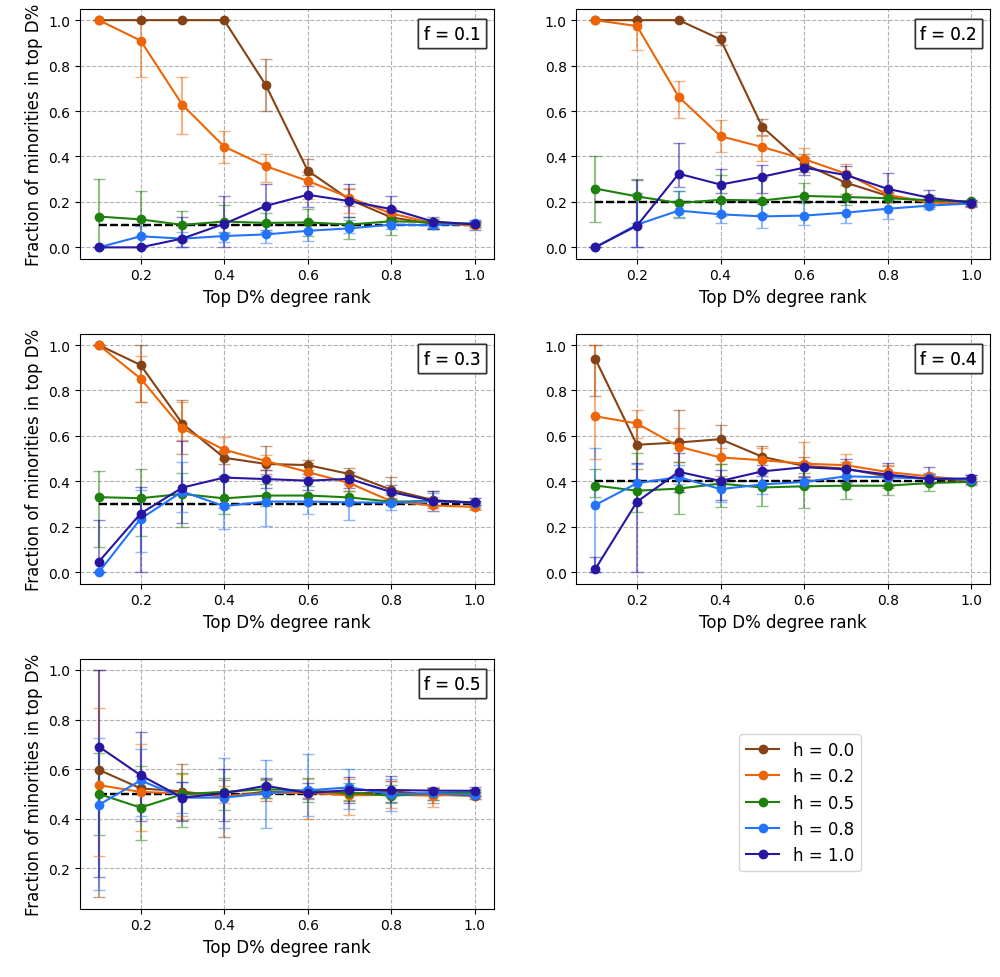
\includegraphics[trim=0 10 0 5, clip, width=1.0\textwidth]{images/top_growth_top00.png}
	\caption{The fraction of minority nodes found in top D\% nodes ranked according to degree in growing networks with \textbf{Top-Rank ($r = 0.0$)}. A black dotted line at each plot shows the actual fraction of minority nodes in the network.}
	\label{top_growth_top00_fig}
\end{figure}

%\section{Experimental Results : Top-Rank (r=0.5)}

\begin{figure}[h!]
	\centering
	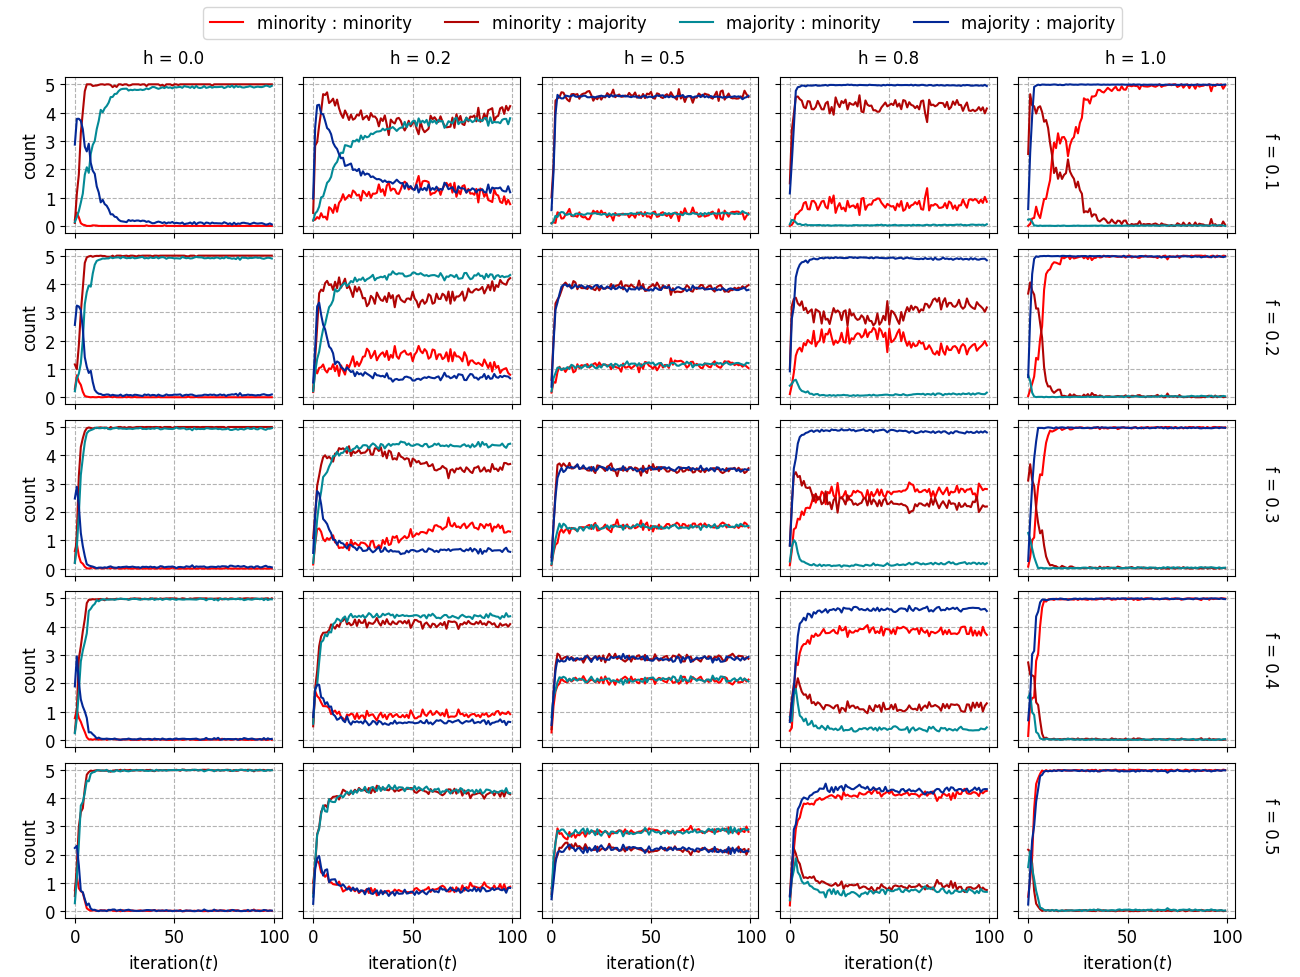
\includegraphics[width=1.0\textwidth]{images/count_top05.png}
	\caption{Count of nodes in the recommendation list over time for minority and majority nodes in a growing network aided with \textbf{Top-Rank}(r=0.5) recommender agent. Homophily values are specified above the respective columns and minority fractions are specified at the right side of the row. Light red plot line denotes count of minority nodes recommended for other minority nodes. Dark red plot line denotes count of majority nodes recommended for other minority nodes. Light blue line denotes count of minority nodes recommended for other majority nodes. Dark blue line denotes count of majority nodes recommended for other majority nodes.}
	\label{count_top05}
\end{figure}

\begin{figure}[h!]
	\centering
	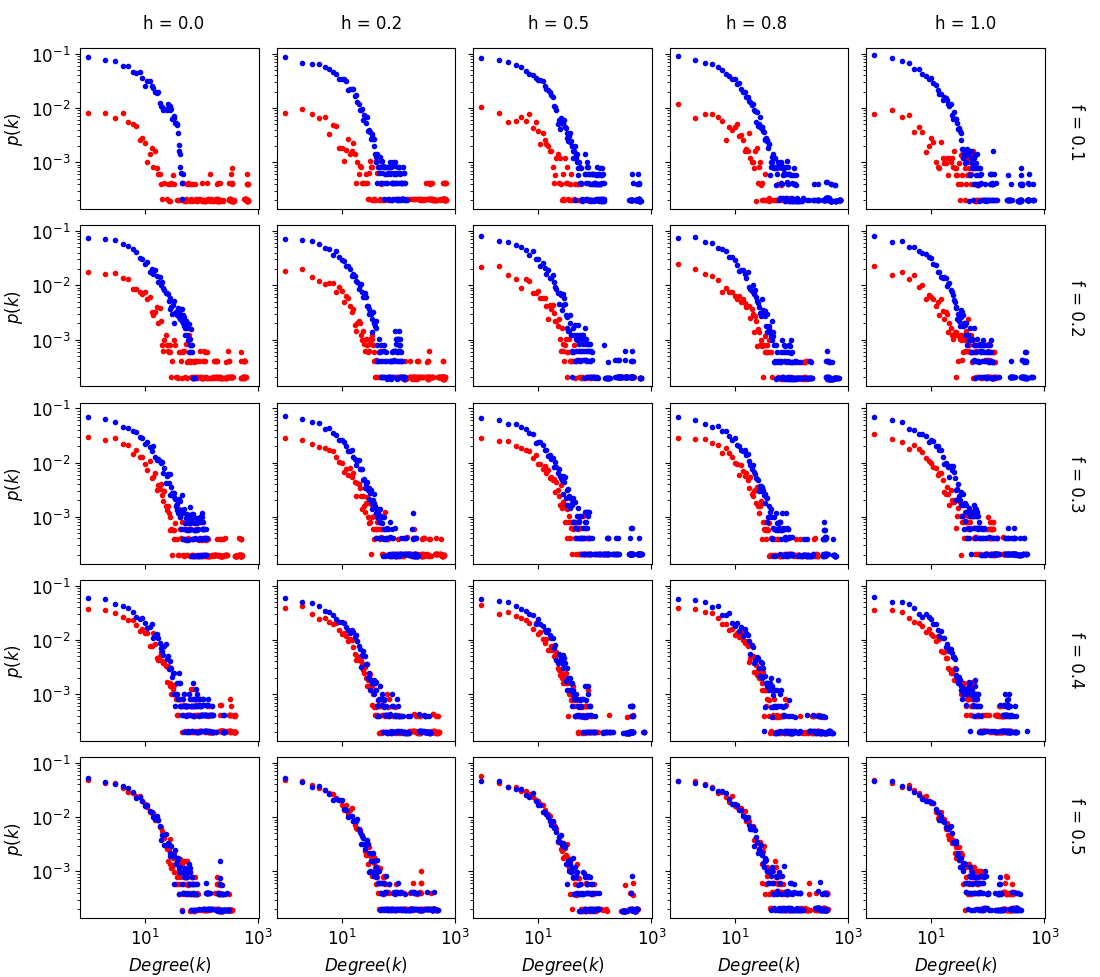
\includegraphics[width=1.0\textwidth]{images/dd_growth_top05.png}
	\caption{Degree distribution for growing networks with \textbf{Top-Rank ($r = 0.5$)}. The minority fractions are provided at the right-side of each row and the homophily values are specified at the top of each column. Degree distribution for the majority and minority nodes are visualized using blue and red plot points respectively.}
	\label{dd_growth_top05_fig}
\end{figure}

\begin{figure}[h!]
	\centering
	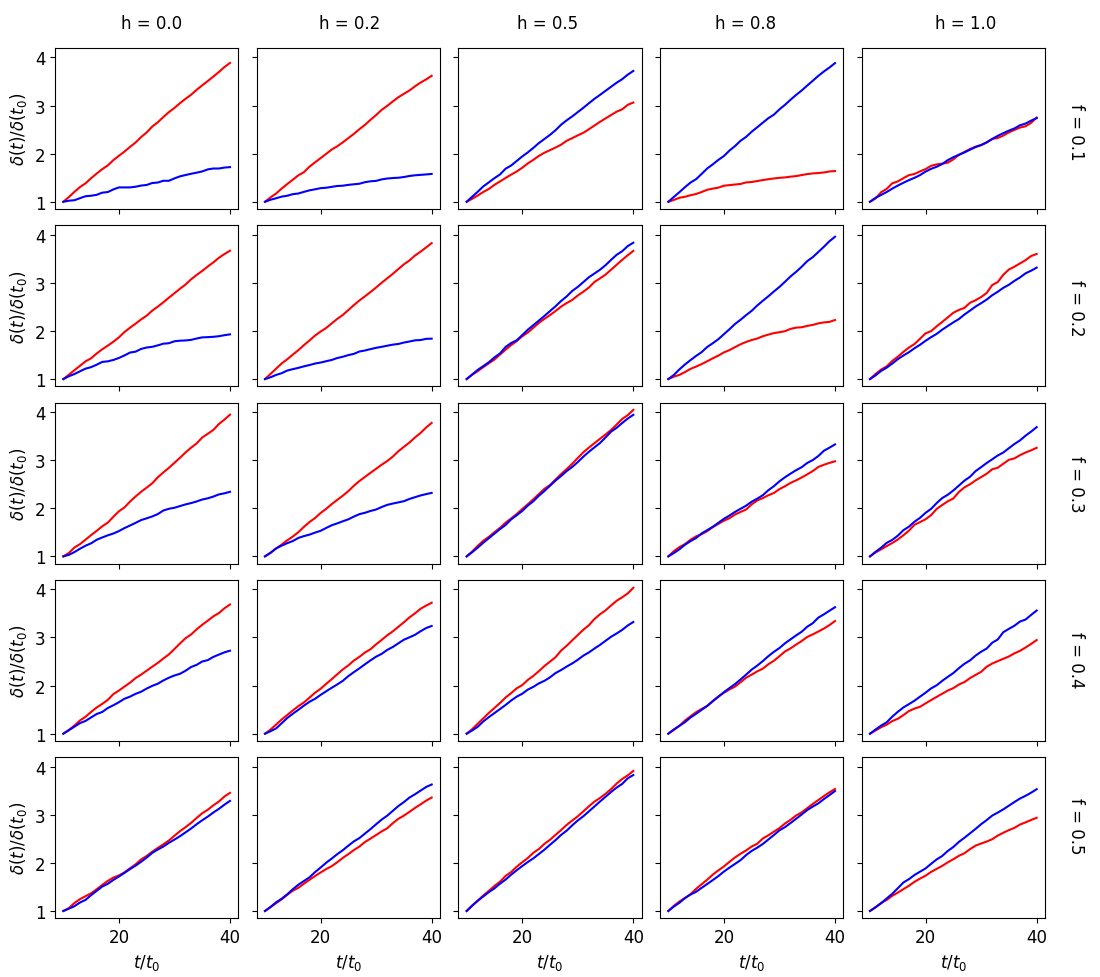
\includegraphics[width=1.0\textwidth]{images/dg_growth_top05.png}
	\caption{Degree growth for growing networks with \textbf{Top-Rank ($r = 0.5$)}. The minority fractions are provided at the right-side of each row and the homophily values are specified at the top of each column. Degree growth for minority and majority node is visualized using red and blue color plot lines respectively.}
	\label{dg_growth_top05_fig}
\end{figure}

\begin{SCfigure}[1][h!]
	\centering
	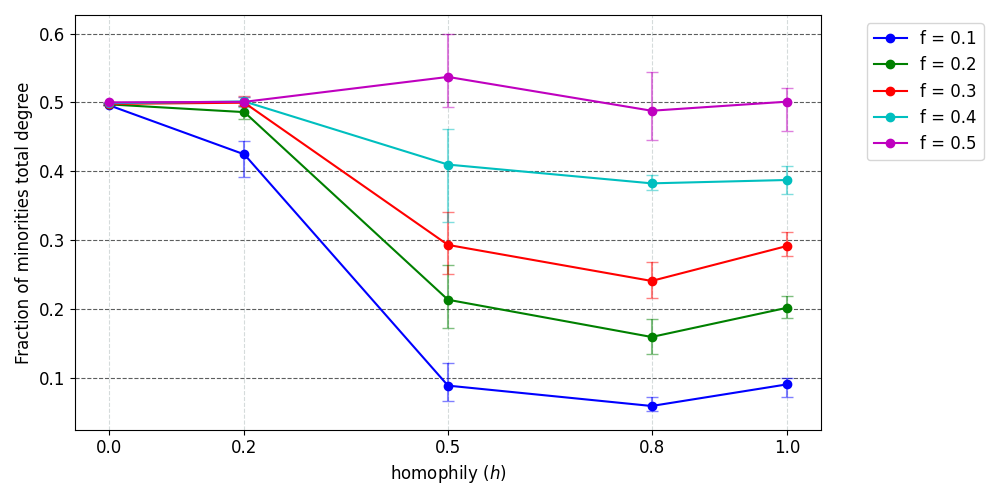
\includegraphics[trim=0 5 0 10, clip, width=0.75\textwidth]{images/mf_growth_top05.png}
	\caption{The fraction of total degree held by minority nodes for growing networks with \textbf{Top-Rank ($r = 0.5$)}.}
	\label{mf_growth_top05_fig}
\end{SCfigure}

\begin{figure}[h!]
	\centering
	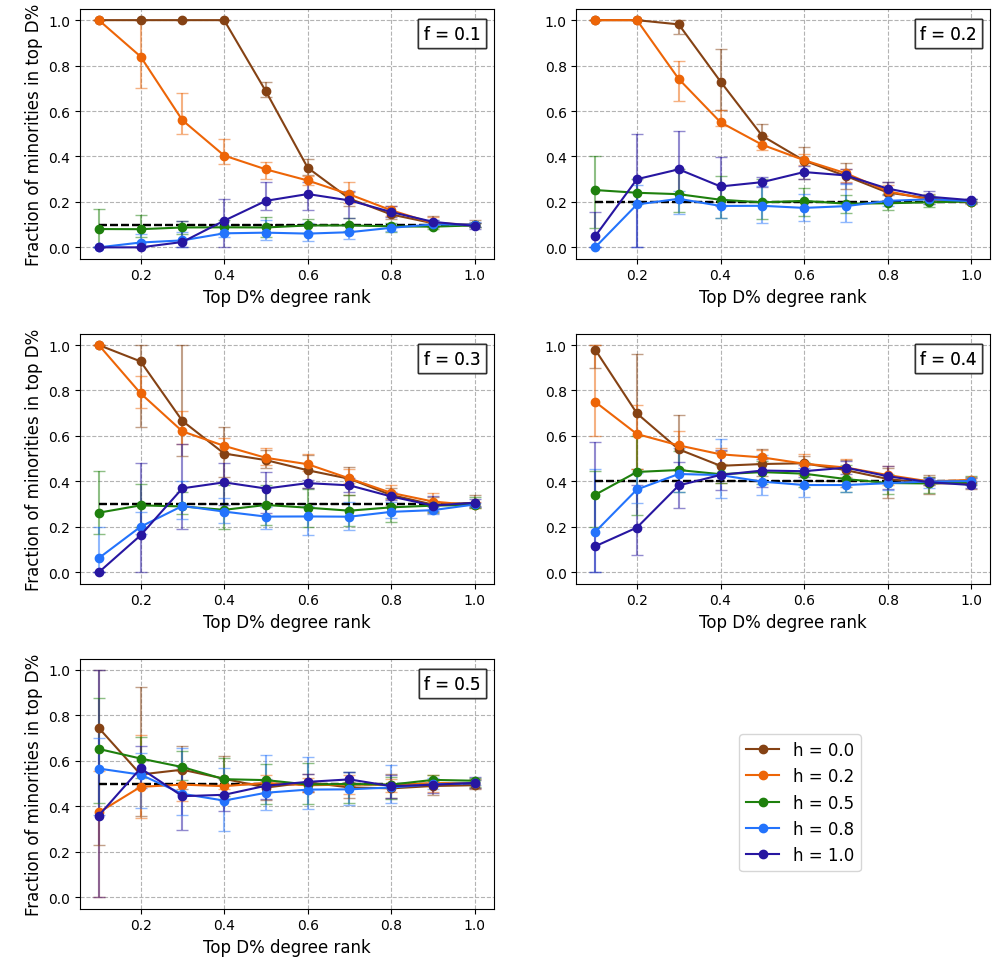
\includegraphics[trim=0 10 0 5, clip, width=1.0\textwidth]{images/top_growth_top05.png}
	\caption{The fraction of minority nodes found in top D\% nodes ranked according to degree in growing networks with \textbf{Top-Rank ($r = 0.5$)}. A black dotted line at each plot shows the actual fraction of minority nodes in the network.}
	\label{top_growth_top05_fig}
\end{figure}

%\section{Experimental Results : Top-Rank (r=1.0)}

\begin{figure}[h!]
	\centering
	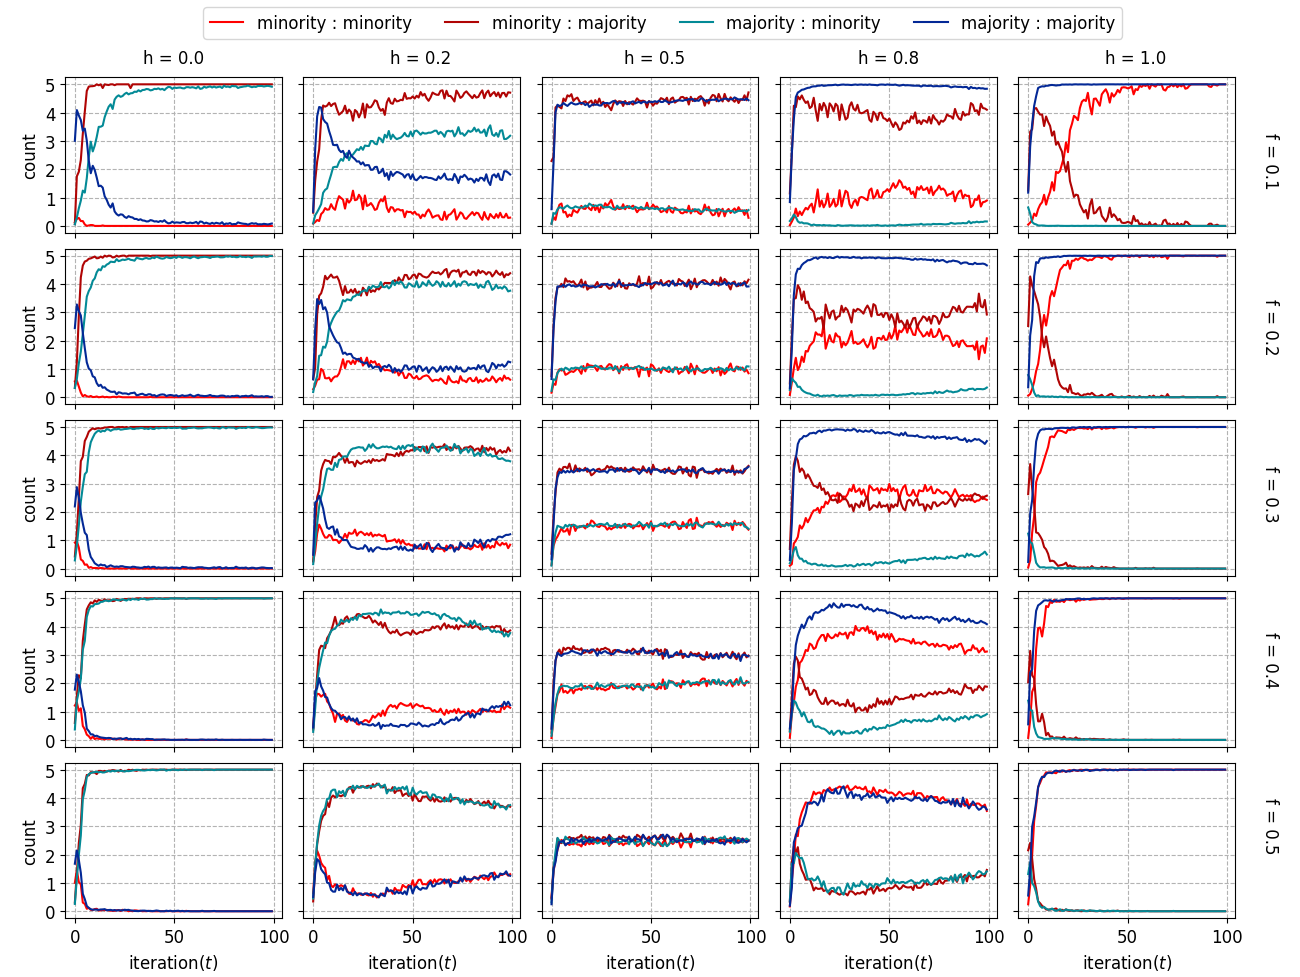
\includegraphics[width=1.0\textwidth]{images/count_top10.png}
	\caption{Count of nodes in the recommendation list over time for minority and majority nodes in a growing network aided with \textbf{Top-Rank}(r=1.0) recommender agent. Homophily values are specified above the respective columns and minority fractions are specified at the right side of the row. Light red plot line denotes count of minority nodes recommended for other minority nodes. Dark red plot line denotes count of majority nodes recommended for other minority nodes. Light blue line denotes count of minority nodes recommended for other majority nodes. Dark blue line denotes count of majority nodes recommended for other majority nodes.}
	\label{count_top10}
\end{figure}

\end{appendices}